\section{Introduction}
\subsection{Purpose}
\hspace*{0.7in} The purpose of this section is to describe "A Tool For Managing Key Value Pairs on Oracle NoSQL". This document contains the functional and non-functional requirements of the project. The recent problem of exponentially growing data and to store and manage is needed to be solved. As a solutions new technologies are been introduced in the market by various vendors. But again using these technologies needs trainings to users. As these technologies does not resemble in any way with the traditional technologies. So the purpose is to make this new introduced Oracle NoSQL, familiar with the user by providing various tools to manage this database for user's purpose.

\subsection{Project Scope}
\hspace*{0.7in} A Tool for Managing Key Value Pairs on Oracle NoSQL is basically a application through which the user can make fundamental operations on Oracle NoSQL Database. Project provides various CRUD functions and Import and Export. Here user has to provide the key and its value either one by one or into chunk from CSV File. The project also provides RESTFul web services which provide all the functionalities for managing Oracle NoSQL Database. The project has an Android Application which is used for Attendance check for the users of particular organization. The application can be used in:
\begin{enumerate}
  \item Performing basic operations on Oracle NoSQL Database.
  \item Into an organization where Oracle NoSQL is used.
  \item The RESTFul web services can be used by any application which needs to use the Oracle NoSQL Database functionalities.
  \item The Attendance check application can be used by organizations having Biometric thumb scan machine for attendance.
\end{enumerate}

\subsection{Need}
\hspace*{0.7in} The system is needed because Oracle NoSQL database does not have any Command Line Interface or Graphical User Interface for managing the database. So the system provides GUI and RESTFul web services which make the ease to user, to handle the Oracle NoSQL database. The RESTFul web services are intended to provide project functionalities on any platform or any class of user.

\subsection{Benefits}
\hspace*{0.7in} It is stated that any database should provide ease to users to make operations effort less and efficient. So this project is intended to reduce the user's efforts for managing Oracle NoSQL database by providing GUI and RESTFul web services for the same.
\subsection{Objectives}
\hspace*{0.7in} The objective behind implementing this application is to make a tool which could make the interaction of user easier with Oracle NoSQL database. This application is is new access mechanism for managing database. The application provides interactive and intuitive interface to the user. The Project also provides RESTFul web services which can be used on any platform who needs to make use of Oracle NoSQL Database.

\subsection{User Classes and Characteristics}
\hspace*{0.7in} Users of the system might be any person who needs to interact or use the Oracle NoSQL Database. The user must have basic knowledge of the Key Value Pair based Oracle NoSQL database and computer. Administrators of the system must have more knowledge about the internal modules of the system and are able to rectify small problems that may arise due to disk crashes, network failure, power failure and other catastrophes. Friendly user interface, help options and user guide must be sufficient to educate the user on how to use this product without any problem or difficulties.

\subsection{Operating Environment}
\hspace*{0.7in} The project is an online application, which is deployed on the application server. So the application can be accessed and used from any platform having internet connectivity. The RESTFul web services are free to use on any platform, but mostly the RESTFul web services are intended to use on mobile platform or on the platform where low data is to be handled. And the attendance check application works on Android Platform.

\subsection{Assumptions and Dependencies}
\begin{itemize}
  \item The application is intended to be used for managing big data, the user must have fast internet connectivity on his/ her system.
  \item The user who wants to use the RESTFul web services must know how to use the web services on mobile or any other platform.
  \item The most important is that, any user who needs to use the system must have basic knowledge of the Oracle NoSQL Database.
\end{itemize}

%****************************************************************************************************************************

\section{System Features}
\begin{itemize}
  \item Connect To Store
\begin{figure}[h]
\centering
  % Requires \usepackage{graphicx}
  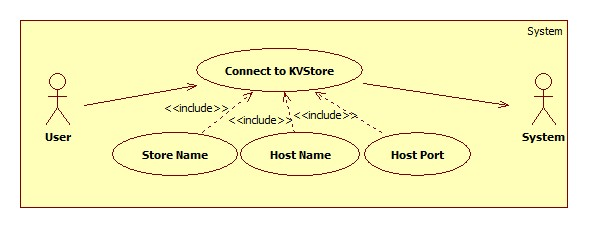
\includegraphics[width=13cm,height=7cm]{Fig1.jpg}
  \caption{Connect To Store}\label{Connect To Store}
\end{figure}
\end{itemize}

\newpage
\begin{itemize}
  \item Insert Data Into Store
\begin{figure}[h]
\centering
  % Requires \usepackage{graphicx}
  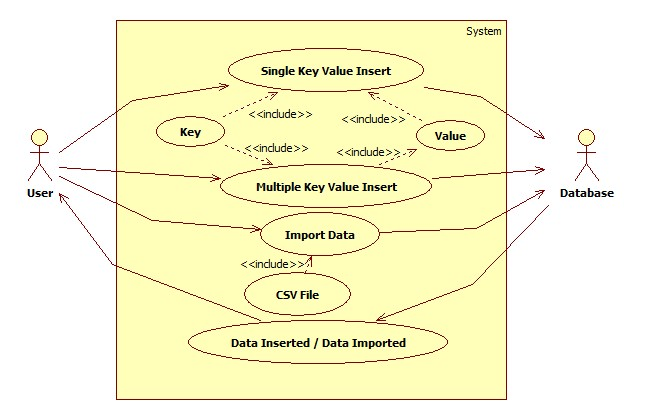
\includegraphics[width=11.5cm,height=8cm]{Fig2.jpg}
  \caption{Insert Data Into Store}\label{Insert Data Into Store}
\end{figure}
\end{itemize}

\begin{itemize}
  \item Display Data
\begin{figure}[h]
\centering
  % Requires \usepackage{graphicx}
  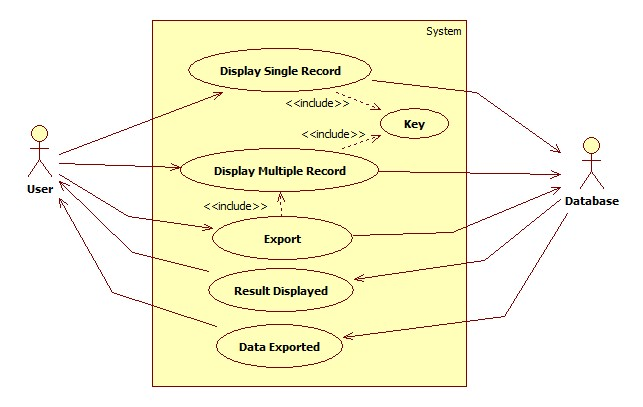
\includegraphics[width=11.5cm,height=8cm]{Fig3.jpg}
  \caption{Display Data}\label{Display Data}
\end{figure}
\end{itemize}

\newpage
\begin{itemize}
  \item Delete Data
\begin{figure}[h]
\centering
  % Requires \usepackage{graphicx}
  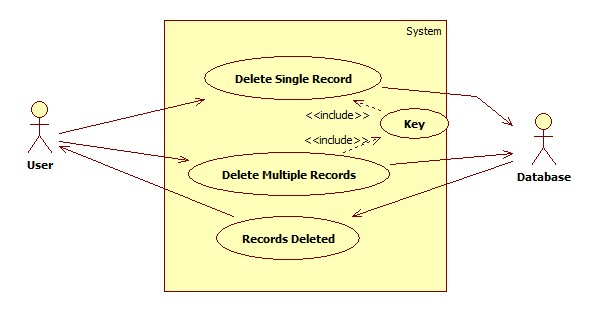
\includegraphics[width=11.5cm,height=9cm]{Fig4.jpg}
  \caption{Delete Data}\label{Delete Data}
\end{figure}
\end{itemize}

\begin{itemize}
  \item Update Data
\begin{figure}[h]
\centering
  % Requires \usepackage{graphicx}
  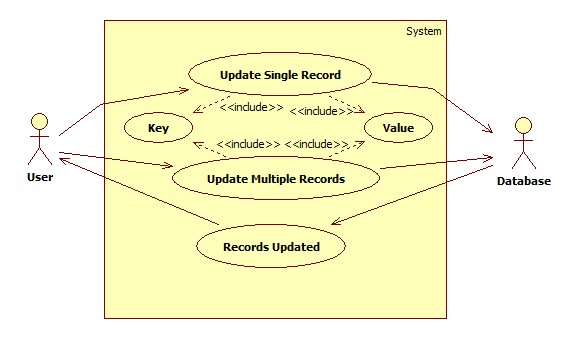
\includegraphics[width=11.5cm,height=7cm]{Fig5.jpg}
  \caption{Update Data}\label{Update Data}
\end{figure}
\end{itemize}

\newpage
\begin{itemize}
  \item Import/Export
\begin{figure}[h]
\centering
  % Requires \usepackage{graphicx}
  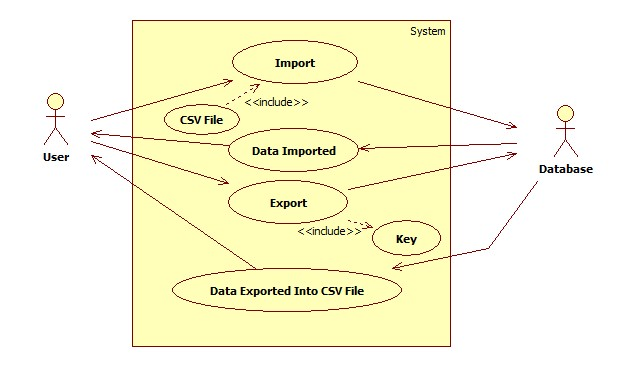
\includegraphics[width=11.5cm,height=8cm]{Fig6.jpg}
  \caption{Import/Export}\label{Import/Export}
\end{figure}
\end{itemize}

\begin{itemize}
  \item Daily Attendance Check
\begin{figure}[h]
\centering
  % Requires \usepackage{graphicx}
  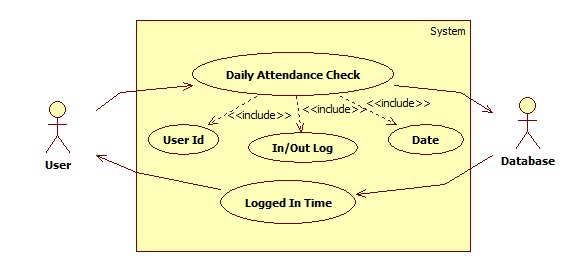
\includegraphics[width=11.5cm,height=7cm]{Fig7.jpg}
  \caption{Daily Attendance Check}\label{Daily Attendance Check}
\end{figure}
\end{itemize}

\newpage
\begin{itemize}
  \item Monthly Attendance Check
\begin{figure}[h]
\centering
  % Requires \usepackage{graphicx}
  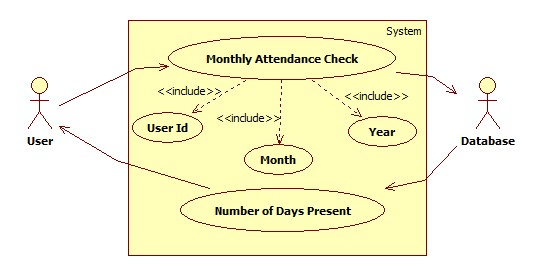
\includegraphics[width=11.5cm,height=7cm]{Fig8.jpg}
  \caption{Monthly Attendance Check}\label{Monthly Attendance Check}
\end{figure}
\end{itemize}

%***************************************************************************************8
\section{External Interface Requirements}
\subsection{User Interfaces}
\begin{itemize}
  \item Home Screen :
\end{itemize}
After starting the application home screen should appears. Home screen has various options including insert, display, update, delete, import and export. But for performing any of this operation the application needs to be connected to the KVStore. For this purpose application asks to user for three options i.e. Store Name, Host Name on which the database is installed and the Host Port on which the database service is running. After getting these parameters the application would connect to database server. And the session for that user should be initialized.

\begin{itemize}
  \item Insert Record :
\end{itemize}
Using this option the user can insert either single Key Value pair or Multiple Key Value pairs into the database. For single Key Value Pair insertion user needs to enter Major Key Component, Minor Key Component and Value. And for multiple Key Value Pairs insertion first user needs to enter Major Key Component and number of Minor Key Component for same, followed by this number of Minor Key Components would have to be inserted and Values for them respectively.

\begin{itemize}
  \item Display Record :
\end{itemize}
This option is used for either single or multiple Key Value Pair display. For single Key Value Pair display user needs to enter the Major Key Component and Minor Key Component of which the value is to be displayed. And for multiple Key Value pairs display user only needs to enter Major Key Component.

\begin{itemize}
  \item Delete Record :
\end{itemize}
This option is used to delete single or multiple Key Value pair from database. For single value deletion user needs to enter Major Key Component and Minor Key Component and for deletion of multiple records user has to enter Major Key Component only.

\begin{itemize}
  \item Update Record :
\end{itemize}
Using this option the user can update the existing records into database. For updating single key value pair user has to enter Major Key Component, Minor Key Component and Value for them. And for updating multiple Key Value pair user has to enter Major Key Component its Minor Key Components and their respected values.

\begin{itemize}
  \item Import :
\end{itemize}
This option should provide the functionality of importing data from CSV file to Oracle NoSQL Database. Here very firstly a CSV file is uploaded to the server. And after that user has to specify Major Key Component and Minor Key Component for that file and user also has to specify that which field from the file is to be relate with Minor Key Component.

\begin{itemize}
  \item Export :
\end{itemize}
Here the user can export the data to CSV file from the database. Very firstly the user has to specify Major Key Component by which he/she would get multiple records and after that user can download that file.

\begin{itemize}
  \item Android Interface for Attendance Check :
\end{itemize}
Using this application the user can check daily as well as monthly attendance. Here the user first needs to connect to database and after that user has to specify userid, In/Out log and date for daily attendance check, and userid, month and year for monthly attendance check.

\subsection{Hardware Interfaces}
\begin{itemize}
  \item Intel Core 2 Duo or higher processor.
  \item Android device with Ginger bread version or higher.
  \item Android device with more than 125 mb RAM.
  \item For deployment of server application the server should be good configuration.
\end{itemize}

\subsection{Software Interfaces}
\begin{itemize}
  \item Any operating system where java can be installed.
  \item Apache tomcat or Glassfish server.
  \item Any Internet browser.
  \item Android operating system.
\end{itemize}

\section{Nonfunctional Requirements}

\subsection{Performance Requirements}
\begin{itemize}
  \item The server must be able to handle all the requests incoming from the clients.
  \item Network bandwidth must be properly managed while the big CSV file is uploaded to the server.
  \item While retrieving multiple Key Value from the database server, the records must be retrieved into batches so that network would not get jammed.
  \item On android device the application must not take more space into internal memory and RAM.
  \item The client must operate at less internet speed.
\end{itemize}

\subsection{Safety Requirements}
\begin{itemize}
  \item UPS: in case of power failure the system requires UPS.
  \item Hard Disk:  the database server must have enough space to store the Data.
  \item The network at the database server side must be properly managed so that it should not crash during the operations are in progress.
\end{itemize}

\subsection{Software Quality Attributes}
\begin{itemize}
  \item Data Security : The data stored at the database server is safe as the Oracle NoSQL takes care of it.
  \item Adaptability : the system must be able to adapt the changes made onto the device. In case if the system software is updated then the application must also adapt those changes.
  \item Availability : availability defines that whenever the application is needed that time user must get the service.
  \item Correctness : every time the data is accessed that time correct data should be provided.
  \item Flexibility : the application should be flexible with any class of user.
  \item Maintainability : the system should not need more maintenance as the end user is not expertise to do so.
  \item Reliable: the user can be reliable on the system, as the system is reliable.
  \item Reusability: the code of application is reusable. The RESTFul web can be reused into other applications.
  \item Robustness: the application can be operate into any device environment.
  \item Testability: the system can be exposed to the test all its functionalities.
\end{itemize}
 %************************************************************************************

\section{Analysis Model}
\subsection{Class Diagrams}
\hspace*{0.7in} Class diagram in the unified modeling language(UML) is a type of static structure  diagram that describes the structure of a system by showing the system's classes, their attributes ,and the relationship between the classes .It is the main building block in object oriented modeling. It is being used for both general conceptual modeling of the systematic of the application, and for detailed modeling translating into programming code \\
\begin{figure}[h]
\centering
  % Requires \usepackage{graphicx}
  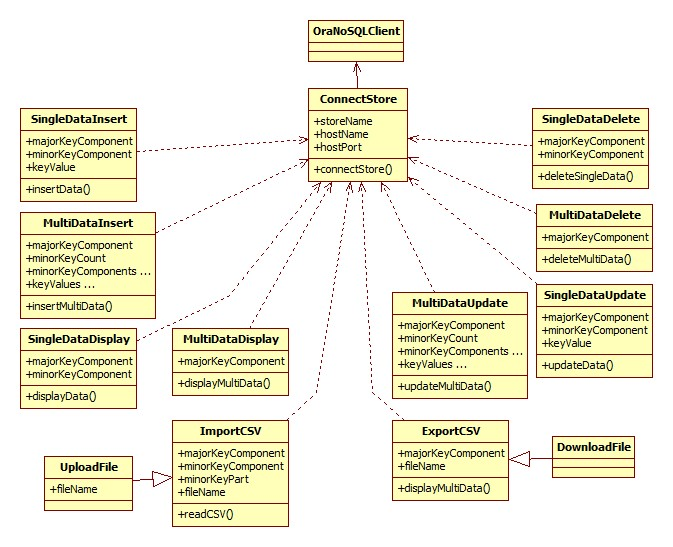
\includegraphics[width=17cm,height=13cm]{Fig9.jpg}
  \caption{Class Diagrams}\label{Class Diagrams}
\end{figure}

\newpage
\section{System Implementation Plan}
There are many important phases for implementation. Following are some important phases and task of implementation.
\begin{itemize}
  \item The main phase to study the NoSQL standard.
  \item Followed by that to Study the Oracle NoSQL and its Architecture in detail.
  \item Understand the use case for which the system is to be implemented.
  \item After understanding the use case proper plan is to created.
  \item So according to plan very first the GUI is to be decided. Various functions will be decided which are to be performed by the system. Based on this function further implementation will be done.
  \item Taking consideration the implementation phase, all the necessary software required for implementation should be installed on the machine.
  \item After the GUI based application is completed, test its functionalities. If all functionalities are up to the mark then proceed to the next phase or remove the errors or bugs.
  \item The next phase is to implement the RESTFul web services. For this purpose, first understand the use case and accordingly start the implementation.
  \item Test the web services, if they are according to use case they move further or again check the functionalities and correct it.
  \item Next step is to implement the Android Application which will consume the RESTFul web services.
  \item After completing the entire above tasks the application is ready to be used.
\end{itemize}

\subsection{Description of Implementation}
\begin{itemize}
  \item The system must be developed into phases as described above.
  \item The system should follow prototype model.
  \item Here none of the prototype depends upon each other, so can be developed in parallel. Development in parallel will reduce the time to develop the project and also the implementation cost.
\end{itemize}

